%%%%%%%%%%%%%%%%%%%%%%%%%%%%%%%%%%%%%%%%%%%%%%%%%%%%%%%%%%%%%%%%%
\chapter{EXPERIMENTS}
\label{ch:CH5}
%%%%%%%%%%%%%%%%%%%%%%%%%%%%%%%%%%%%%%%%%%%%%%%%%%%%%%%%%%%%%%%%%

All the code developed for the experiments explained in this section can be found on master branch of the \verb|GitHub| public repository: \newline
\textcolor{blue}{\hyperrefurl{https://github.com/ozanguldali/modelsWithLASSO}}.
h
\href{https://www.python.org/downloads/release/python-376/}{\texttt{Python}} programming language (version of 3.7.6) along with \href{https://releases.llvm.org/4.0.1/}{\texttt{Clang}} (version 4.0.1) was used to train, test, and classify data in our environment. \href{https://pytorch.org/get-started/previous-versions/#v150}{\texttt{PyTorch}} module with the torch version of 1.5.0, the torchsummary version of 1.5.1 and the torchvision version of 0.6.0, and \href{https://scikit-learn.org/stable/whats_new/v0.23.html}{\texttt{scikit-learn}} library with the version of 0.23.2 were used for implementation of CNN and ML algorithms, respectively. All experiments were performed on the \href{https://colab.research.google.com/}{\texttt{Google Colaboratory}} using its GPU with the number of workers as four.

The construction stages of the experiments we aim to carry out in the thesis can be listed as follows:

\begin{enumerate}
	\item Determine the problem to study,
	\item Explore the data source and choose the one containing appropriate samples  for the determined problem, which is a chest X-ray image data source consisting of COVID-19 samples and non-COVID-19 samples and including the demographic information of samples for our study,
	\item Know and understand the data source, and define classes,
	\item Determine the rules to construct the data set for experiments by cleaning the samples from data source, then construct the data set and divide it into train and test sets containing each class, \label{dividing_step}
	\item Do CNN experiments on different pre-trained models with different transfer learning strategies and with different optimizers, then save the results and model weights to distinct files,
	\item Choose the best results for each model, and use their model weight files to extract the deep features of images in dataset, say $X_{cnn}$,
	\item Do ML experiments using grid search to reach the optimal hyper-parameters on different models over $X_{cnn}$ feature matrix with two methodologies: 1) apply cross-validation only on train set separated in step (\ref{dividing_step}) to yield the generalized results, and 2) train on train set and test on test set separated in step (\ref{dividing_step}) to yield the results for predetermined test set, \label{ML_experiment_step}
	\item Extract the demographic information from dataset for each sample, and construct the demographic information feature matrix, say $X_{info}$,
	\item Do ML experiments using grid search to reach the optimal hyper-parameters on different models over $X_{info}$ feature matrix with two methodologies: 1) apply cross-validation only on train set separated in step (\ref{dividing_step}) to yield the generalized results, and 2) train on train set and test on test set separated in step (\ref{dividing_step}) to yield the results for predetermined test set,
	\item Combine feature matrices $X_{cnn}$ and $X_{info}$ column-wise to construct the feature matrix for each sample, say $X_{all}$, i.e. the feature matrix consisting of the deep features of image data and demographic information of each sample,
	\item Do ML experiments using grid search to reach the optimal hyper-parameters on different models over $X_{all}$ feature matrix with two methodologies: 1) apply cross-validation only on train set separated in step (\ref{dividing_step}) to yield the generalized results, and 2) train on train set and test on test set separated in step (\ref{dividing_step}) to yield the results for predetermined test set, and
	\item Report all results of experiments.
\end{enumerate}

\section{Data Set}

The data was obtained from a public \texttt{GitHub} repository which can be reached via the link \textcolor{blue}{\hyperrefurl{https://github.com/ieee8023/covid-chestxray-dataset/}}. On the GitHub repository, the general information about data is in \href{https://github.com/ieee8023/covid-chestxray-dataset/blob/master/metadata.csv}{\texttt{metedata.csv}} file and the image data is available under \href{https://github.com/ieee8023/covid-chestxray-dataset/tree/master/images}{\texttt{images}} folder.

To construct the data set, the \texttt{metedata.csv} file was parsed and the tabular data were filtered depending on whether it has age and sex information or not, its finding includes the word "COVID-19" term or not, its modality is "X-ray" or not, and its view is "PA" or not. First, data having sex and age information, modality as "X-ray", and view as "PA" were chosen. Then two main classes were constructed by separating the chosen data whether its finding includes "COVID-19" or not. The data including "COVID-19" in its finding were labeled as "COVID-19" and the others were labeled as "non-COVID-19". At the end, there were a total of 131 "COVID-19" and 123 "non-COVID-19" labeled data. An example for "COVID-19" and "non-COVID-19" labeled data can be seen in Figure~\ref{fig:dataset_samples}. Afterwards, with the ratio of 80 to 20, the labeled data were divided into train and test data sets with approximate sizes, 203 and 51, respectively. While the train set now includes 105 "COVID-19" and 98 "non-COVID-19" labeled data, the test data set now includes 26 "COVID-19" and 25 "non-COVID-19".



\begin{figure}[h]
	\centering
	\subfigure[Image labeled as COVID-19. ]{\label{fig:dataset_samples_a}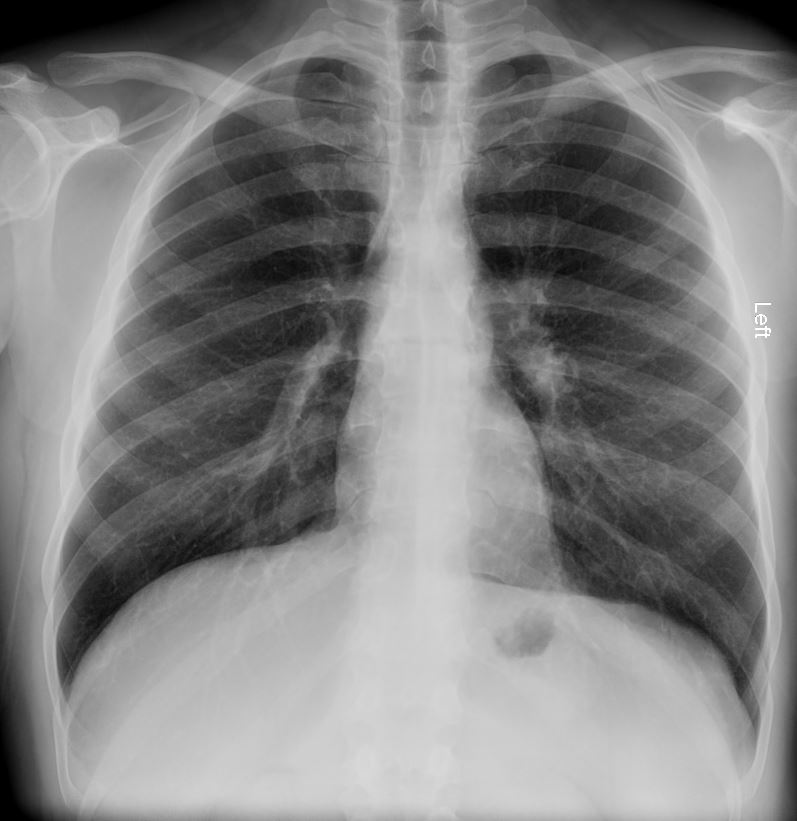
\includegraphics[width=.4\linewidth,height=.4\linewidth,scale=0.6]{fig/train_covid_data.jpg}}
	\subfigure[Image labeled as non-COVID-19.]{\label{fig:dataset_samples_b}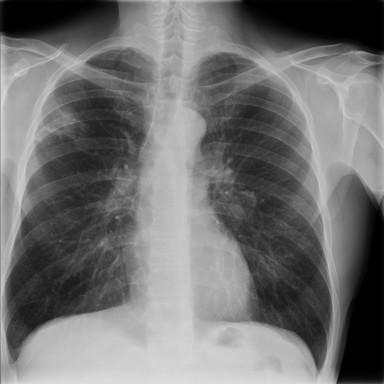
\includegraphics[width=.4\linewidth,height=.4\linewidth,scale=0.6]{fig/test_non_covid_data.jpg}}
	\caption{Data set samples.}
	\label{fig:dataset_samples}
\end{figure}

Image data were appeared in different formats such that .png, .jpg, .jpeg, with different aspect ratios and dimensions such as $384 \times 384$, $462 \times 450$, etc, and in different sizes such as 606 KB, 69 KB, 1 KB, etc. Thus, before using the data, each datum was resized to $224 \times 224$, center cropped, gray scaled, and normalized by the mean of (0.485, 0.456, 0.406) and the standard deviation of (0.229, 0.224, 0.225) for red, blue and green channels respectively. The described process can be seen with an example in the Figure ~\ref{fig:data_transform_steps}. 

\begin{figure}[h]
	\centering
	\subfigure[Original (826×768)]{\label{fig:data_transform_steps_a}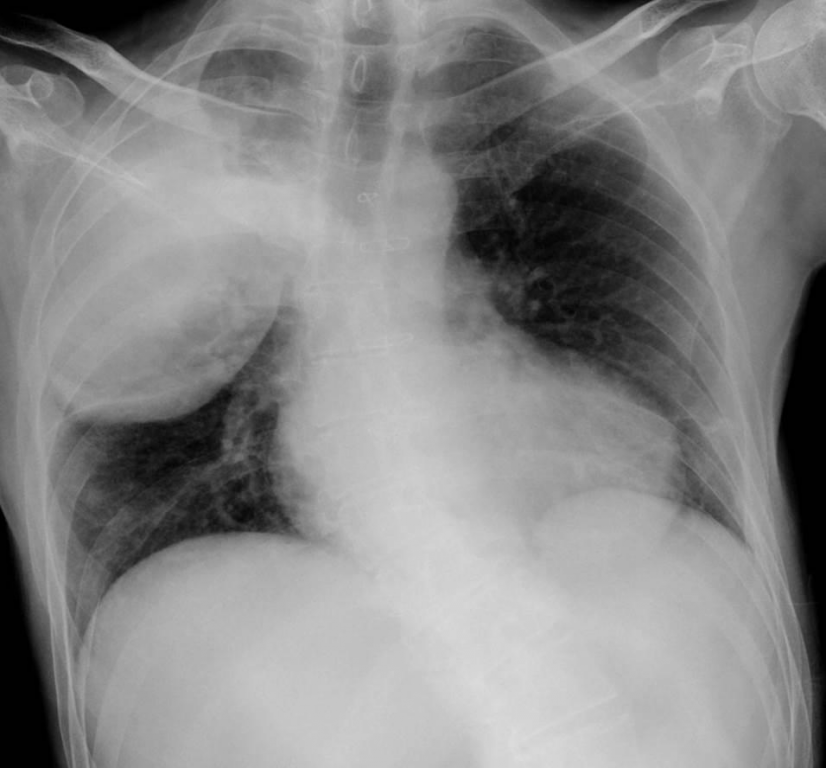
\includegraphics[width=.35\linewidth]{fig/test_covid_data.jpg}}
	\subfigure[Resized, square cropped and gray-scaled]{\label{fig:data_transform_steps_b}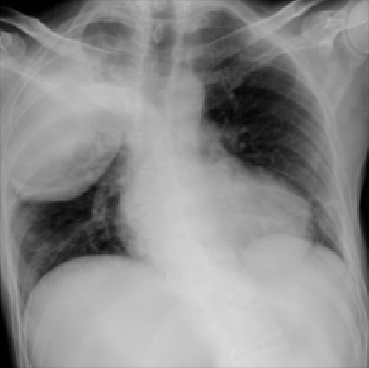
\includegraphics[width=.25\linewidth]{fig/test_covid_data_cropped.png}}
	\subfigure[Normalized]{\label{fig:data_transform_steps_c}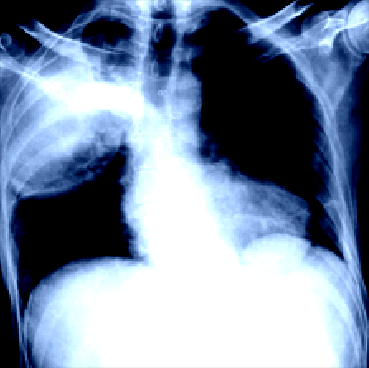
\includegraphics[width=.25\linewidth]{fig/test_covid_data_cropped_normalized.png}}
	\caption{Image transformation steps - Test COVID-19 sample.}
	\label{fig:data_transform_steps}
\end{figure}

\section{Data Augmentation}

Since class sizes are unbalanced, one or more data augmentation techniques are used on train data to balance the class sizes. Furthermore, even for a balanced data set, one can use data augmentation to increase the train data size.

Data augmentation techniques on visual data can be classified in two groups such that position augmentation and color augmentation. Position augmentation takes the original data and applies the desired operations from followings: flipping, rotation, translation, and scaling. On the other hand, during the color augmentation, the augmented datum is obtained by changing one or more of followings: hue, saturation, brightness and contrast. If n kind augmentation choice is used to m number of data, at the end m*(n+1) data are obtained. That is the summation of n augmented datum for each sample of m data, and the original m samples.

In the thesis,  position augmentation, that can be seen via an example in Figure~\ref{augmented_sample}, including horizontal flip,  vertical flip,  90 degrees of rotation, 180 degrees of rotation, and 270 degrees of rotation is used on the whole train data. These augmented data are not physically available, i.e. not saved as files, and only used throughout CNN training process. Data augmentation is not used on ML processes.

The number of data on train and test sets for each class after data augmentation can be seen in Table~\ref{tab:final_dataset_size}.

\begin{table*}[h]
	{
		\setlength{\tabcolsep}{14pt}
		\caption{The distribution of class sizes across train (including augmented train set) and test sets.}
		\begin{center}
			% \vspace{-6mm}
			\begin{tabular}{lccrrrrr}
				\hline
				\multirow{2}{*}{\textbf{Class}} & \multirow{2}{*}{\textbf{Original Set}} & \multicolumn{2}{c}{\textbf{Train Set}} & \multirow{2}{*}{\textbf{Test Set}} \\ \cline{3-4}
				&                               & \textbf{Chosen}  & \textbf{Augmented}  &    \\
				\hline \hline
				COVID-19           & 131                           & 105     & \multicolumn{1}{c}{630} & \multicolumn{1}{c}{26} \\
				Non-COVID-19               & 123                           & 98      & \multicolumn{1}{c}{588} & \multicolumn{1}{c}{25} \\
				TOTAL                  & 254                           & 203     & \multicolumn{1}{c}{1218} & \multicolumn{1}{c}{51} \\   
				\hline
			\end{tabular}
			% \vspace{-6mm}
		\end{center}
		\label{tab:final_dataset_size}
	}
\end{table*}

\begin{figure}[h]
	\centering
	\subfigure[Original Sample ]{\label{fig:augmented_sample_a}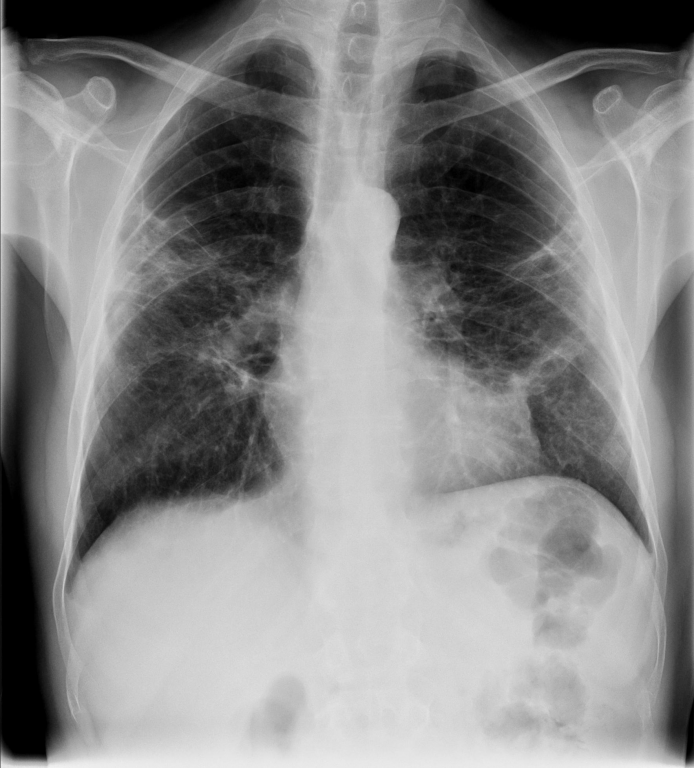
\includegraphics[width=.3\linewidth]{fig/train_non_covid_data.jpg}}
	\subfigure[Horizontal flipped]{\label{fig:augmented_sample_b}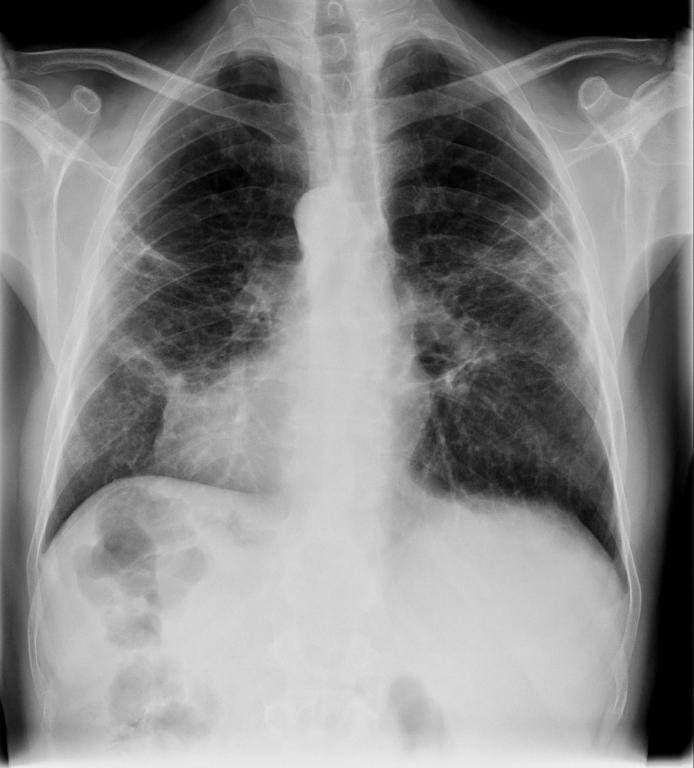
\includegraphics[width=.3\linewidth]{fig/horizontalFlipped_train_non_covid_train_data.jpg}}
	\subfigure[Vertical flipped]{\label{fig:augmented_sample_c}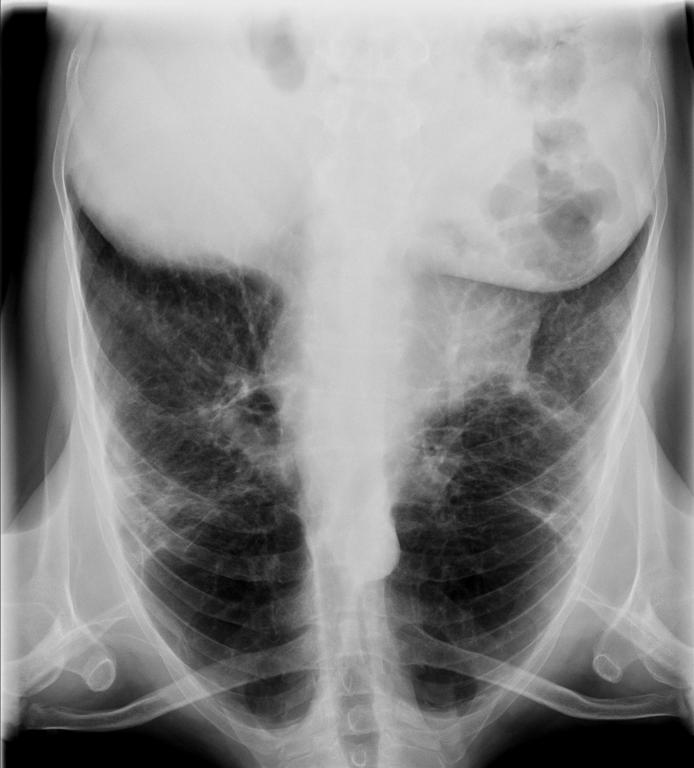
\includegraphics[width=.3\linewidth]{fig/verticalFlipped_train_non_covid_train_data.jpg}}
	\subfigure[90 degrees rotated]{\label{fig:augmented_sample_d}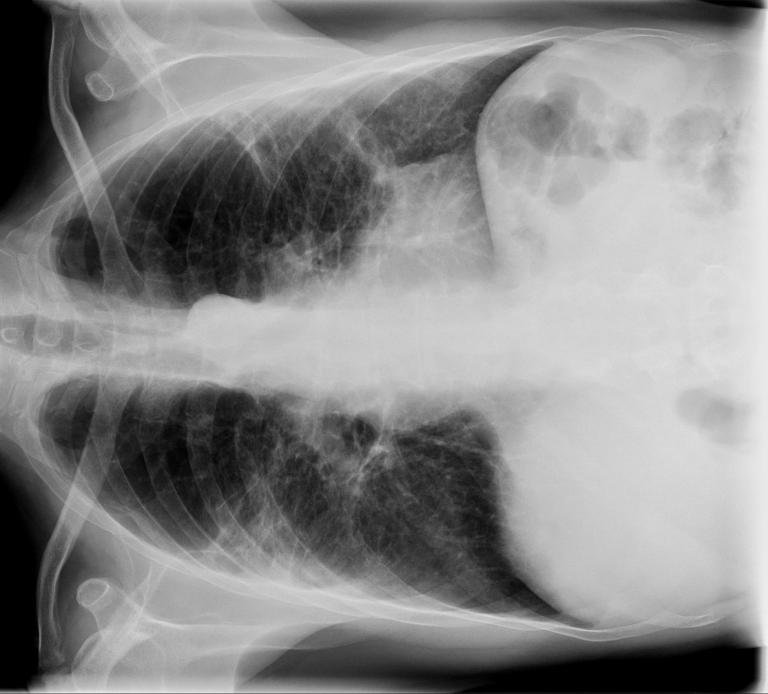
\includegraphics[width=.3\linewidth]{fig/90Rotated_train_non_covid_train_data.jpg}}
	\subfigure[180 degrees rotated]{\label{fig:augmented_sample_e}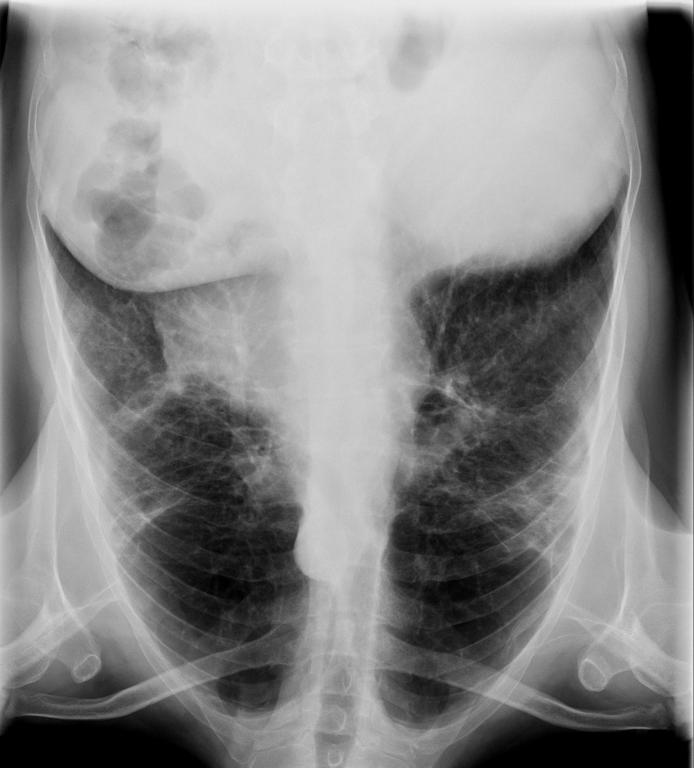
\includegraphics[width=.3\linewidth]{fig/180Rotated_train_non_covid_train_data.jpg}}
	\subfigure[270 degrees rotated]{\label{fig:augmented_sample_f}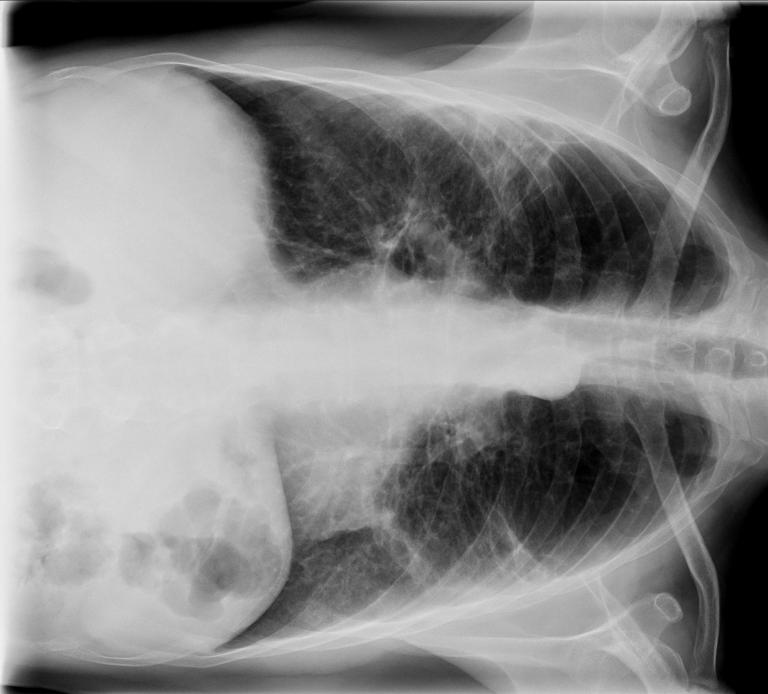
\includegraphics[width=.3\linewidth]{fig/270Rotated_train_non_covid_train_data.jpg}}
	\caption{An original non-COVID-19 and sample from train data set and position augmentations applied.}
	\label{augmented_sample}
\end{figure}

\newpage

\section{Training and Testing with Convolutional Neural Network Models}\label{sec:CH5_cnn_experiments}

All CNN experiments used in this thesis was performed on pre-trained CNN models which are AlexNet, ResNet-18, ResNet-34, ResNet-50, VGG16, and VGG19. In other words, the appropriate model weights were used with different strategies explained in Section~\ref{CH3:transfer_learning} to feed the models.

Since our data set is small and the data content is different from ImageNet dataset \cite{imagenet}, we experimented two different transfer learning strategies such that the first is to train the entire model, and the second is to freeze the first few layers and train others. The frozen layers on the second strategy for each experiment model are:

\begin{itemize}
	\item The first convolution layer and the following ReLU and maximum pooling layers for AlexNet architecture,
	\item The first convolution layer and the following batch normalization, ReLU, and maximum pooling layers for ResNet architectures, and
	\item The first six layers which are in order of convolution, batch normalization, ReLU, convolution, batch normalization, ReLU, and maximum pooling layers for VGG architectures.
\end{itemize}

Throughout the study, our experience and earlier comparison results, which are not reported here, have shown that training the entire model instead of freezing the associated layers discussed above for the corresponding architectures gives more minimal losses and more accurate classification results. However, it must be remarked that, even the number of frozen layers are not high, since the number of parameters is smaller in freezing approach than the number of parameters in training the entire model, the computation time of each batch is observably shorter in freezing approach.

Train data were set to be shuffled at each epoch and the batch size was experimentally set from $2^4$ to $2^6$. The number of epochs was set to 50 and the validation period was set as $1/50$. In other words, before the first training epoch and after each training epoch, validation process was applied on test set. On each validation, the saved model weights files for the corresponding configurations were checked. If there exists no saved file having greater accuracy percentage than the current state, the current model weights are saved as a new model weight *.pth file with the name including the validation result and training configurations. The saved CNN model weights files can be found under the \textit{/cnn/saved\_models} directory of project repository at \textcolor{blue}{\hyperrefurl{https://github.com/ozanguldali/modelsWithLASSO}}. After the last training epoch, testing process is applied rather than validation, and the same accuracy comparison over saved *.pth files is executed. That is why, the number of validation accuracy results are 50 whereas the number of validation losses are 49. The reason why we limited the epoch size to 50 is that the models were over-fitted after this number or even earlier than this number sometimes.

Because of our weights file comparison rule, there may be multiple *.pth weights files for the same configuration and accuracy value. This time, the train loss values, before the validation or test result obtained, and the validation loss values, if available, are considered. Here, the less loss is better to choose.

The cross-entropy loss function, explained in Section~\ref{sec:CH3_cross_entropy}, was used for all CNN models. To optimize it, SGD momentum, Adam, and AdamW optimizers were experimented with various learning rates, momentum values (if applicable), and weight decay parameter values (if applicable). Moreover, the learning rate was experimentally scheduled by the reducing rate as by 0.1 for each quarter of total epoch size. However, the scheduler approach drove the models to be over-fitted. 

Final hyper-parameters that are accepted as the best for each model differ under each different optimizer. As an example, the best final hyper-parameters for ResNet-50 model under SGD momentum, Adam, and AdamW optimizers can be seen in Table~\ref{tab:cnn_hyperparameters}. Furthermore, in terms of computational time and obtained losses, we encountered the optimal batch size  as $2^4$ in our experiments. Hence, the number of iterations at each epoch was 77 for augmented train data and 4 for test data which was used both on test and validation processes.

\begin{table}[h]
	\centering
	\caption{Final hyper-parameters for ResNet-50 model.}
	\label{tab:cnn_hyperparameters}
	\begin{tabular}{lccc}
		\hline 
		\multicolumn{1}{c}{\textbf{Optimizer}} & \textbf{Learning Rate} & \textbf{Momentum} & \textbf{Weight Decay} \\ \hline \hline
		SGD Momentum                           & 1e-4                   & 0.9               & -                     \\ 
		Adam                                   & 1e-5                   & -                 & 1e-3                     \\ 
		AdamW                                  & 1e-5                   & -                 & 1e-4   \\  \hline              
	\end{tabular}
\end{table}

All pre-trained CNN models were experimented by setting the final layer output as the class size, i.e. 2. Furthermore, for all architectures experienced in this thesis,  a modification is applied onto the classification section by adding a block of ReLU, drop-out, and fully-connected layers right after the last fully-connected layer to adapt the models for our work.

Let us consider the ResNet-50 model, the total parameters, so the total trainable parameters on full-training, is 25,559,034 for one sample. For an input image in the size of 0.59 MB, forward and backward pass size is 309.48 MB and parameters size is 97.50 MB. Hence, the estimated total size of one iteration on this image is 407.57 MB according to \verb|PyTorch|.

Figure~\ref{fig:resnet50_visualization} describes how the process starts with an input image with the size of $227 \times 227$, how the blocks of ResNet-50 are aligned along with the output visualizations for each block, and how to obtain a class prediction for this sample at the end. The higher resolution version of images in Figure~\ref{fig:resnet50_visualization}, such as the visualizations of convolution blocks, is available at directory \textcolor{blue}{\hyperrefurl{https://github.com/ozanguldali/modelsWithLASSO/blob/master/figures}}.


\begin{landscape}
	\begin{figure}[h]
		\centering
		\includegraphics[width=\linewidth]{fig/resnet50_visualization.png}
		\vspace{1mm}
		\caption{The sample visualization representing one iteration on ResNet-50 architecture and class probability result for COVID-19 labeled data from our dataset. The higher resolution version of image is available at \\  \textcolor{blue}{\hyperrefurl{https://github.com/ozanguldali/modelsWithLASSO/blob/master/figures/resnet50_visual.png}}}
		\label{fig:resnet50_visualization}
	\end{figure}
\end{landscape}

\section{Deep Feature Extraction}

After training, validating, and testing the data set on pre-trained CNN models, the deep feature extraction progress could start. Since the model weight files for the best results according to accuracy were stored, these model weights files were used to extract deep features for the corresponding CNN architectures.

Here, the modifications on CNN models stated at previous subsection show its another purpose. The deep features are extracted from the latest fully-connected layer right before the modified classification block consisting of ReLu, drop-out, and the fully-connected layer. Figure~\ref{fig:modified_classification_blocks} briefly gives the deep feature extraction layer and the modified classification block for simple AlexNet, ResNet and VGG architectures. As it can be seen from Figure~\ref{fig:modified_classification_blocks}, the deep features are extracted from:

\begin{itemize}
	\item the third fully-connected layer for AlexNet architecture,
	\item the first fully-connected layer for ResNet architectures, and
	\item the third fully-connected layer for VGG architectures,
\end{itemize}

which are all framed in red color. 
Afterwards, the deep features extracted from CNN models are used to feed machine learning algorithms to improve the classification success.

\begin{figure}[h]
	\centering
	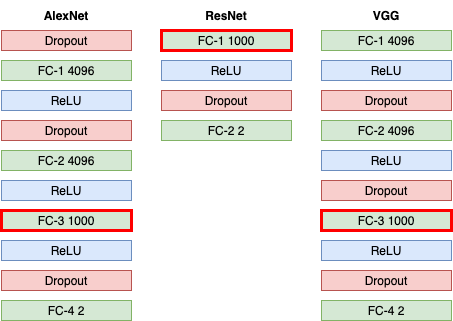
\includegraphics[width=.8\linewidth]{fig/modified_classification_blocks.png}
	\vspace{2mm}
	\caption{Illustration of modified classification blocks for AlexNet, ResNet, and VGG.}
	\label{fig:modified_classification_blocks}
\end{figure}

\section{Forming Feature Matrices} \label{sec:CH5_forming_features}

In this study, we have initially two different types of feature matrices and then we will combine these two to obtain a unique feature matrix. The first feature matrix includes the deep features extracted by the help of CNN models. Instead of image segmentation, Red-Green-Blue (RGB) color codes or manual image partition labeling, we use the features derived from deep learning process. The number of features are 1000 for each CNN architecture because of the output size of fully-connected layers used. We denote the matrix of deep features by $X_{cnn}$ and the feature size is $d_{cnn} = 1000$.

On the other part, we have demographic information, that's age and gender information for each sample. We denote the matrix of demographic information by $X_{info}$ and the feature size as $d_{info} = 2$. Age information was categorized to 5 groups such as under 18, between 18 and 37, between 38 and 59, between 60 and 79, and over 80 ages.

Hence, as can be seen in the Figure~\ref{fig:feature_maps}, the merged feature matrix denoted by $X_{all}$ has the feature size as $d_{all} = 1002$, where the number of rows, N, is 254 in our study.

\begin{figure}[h]
	\centering
	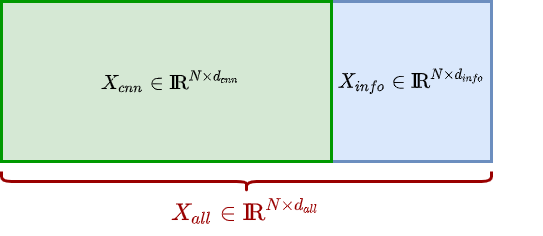
\includegraphics[width=.6\linewidth]{fig/feature_maps.png}
	\vspace{2mm}
	\caption{Feature maps where $d_{cnn} = 1000$, $d_{info} = 2$, and $d_{all} = d_{cnn} + d_{info} = 1002$.}
	\label{fig:feature_maps}
\end{figure}

\section{Data Pre-Processing}

\subsection{Data Standardization}

Machine learning algorithms commonly requires data standardization; because, the data may not be always in the form of standard normal distribution. There are three basic ways to standardize the data such as 1) centering data with the mean, 2) scaling data with the standard deviation, and 3) centering and scaling data with the mean and standard deviation. In the experiments, we only centered the data through the formula given below:
\be
\label{eq:data_standardization}
Z = (X - \mu * I) / \sigma\:,
\ee

where $\mu$ is the mean of training samples and $\sigma$ is set as 1. 


\subsection{Data Normalization}

Data normalization scales each individual sample to have a real value in the unit interval [0.0, 1.0]. Two ways of normalization was experimented which are least absolute technique, known as L1 normalization, and least squares technique, known as L2 normalization.

\begin{itemize}
	\item \textbf{L1 Norm:} Scales the sum of the absolute differences of each individual feature for a sample to 1. That is, it scales the $S_{{L1}_{k}}$ to 1 in the equation (\ref{eq:data_l1_norm}):
	
	\be
	\label{eq:data_l1_norm}
	S_{{L1}_{k}} = \sum_{i=1}^{d} \big|y_{k} - X_{k,i}\big|\:,
	\ee
	
	where d is the number of features, $X_{k}$ is the $k^{th}$ sample ($k=1,\ldots,N$) and $X_{k,i}$ is the $i^{th}$ feature value of corresponding sample, and $y_{k}$ is the target value for corresponding sample. Here, the scaling ratio is $1 / S_{{L1}_{k}}$; thus, $X_{k} / S_{{L1}_{k}}$ gives the L1 normalized feature values for this sample.
	
	\item \textbf{L2 Norm:} Scales the sum of the squares of differences of each individual feature for a sample to 1. That is, it scales the $S_{{L2}_{k}}$ to 1 in the equation (\ref{eq:data_l2_norm}):
	
	\be
	\label{eq:data_l2_norm}
	S_{{L2}_{k}} = \sum_{i=1}^{d} \big(y_{k} - X_{k,i}\big)^{2}\:,
	\ee
	
	where d is the number of features, $X_{k}$ is the $k^{th}$ sample ($k=1,\ldots,N$) and $X_{k,i}$ is the $i^{th}$ feature value of corresponding sample, and $y_{k}$ is the target value for corresponding sample. Here, the scaling ratio is $\sqrt{1 / S_{{L2}_{k}}}$; thus, $X_{k} / \sqrt{S_{{L2}_{k}}}$ gives the L2 normalized feature values for this sample.
\end{itemize}

We used the L2 normalization as the final settings of the data pre-processing pipeline.

\newpage

\section{Hyper-Parameter Tuning}

For each machine learning algorithm, there exists several hyper-parameters and these hyper-parameter settings cannot be generalized since they differ for each problem and data set. For that reason, finding the optimal combination of hyper-parameters is a separate mission. When choosing the most optimal hyper-parameter combinations, which characteristics should be looked for totally depends on the problem and the researcher. In this thesis, we made decision according to accuracy values.

There are three common hyper-parameter optimization methods in machine learning such that grid search, random search, and Bayesian optimization.

\begin{itemize}
	
	\item \textbf{Grid Search:} All combinations between hyper-parameter options are experimented. For instance, if there exists $m$ number of hyper-parameters and each of them has $a_{i}$ options where $a_{i}$'s are positive integers for $i \in \{1,2,\dots,m\}$, then the total number of grid search iterations are $\prod_{i=0}^{m} a_{i}$. Moreover, if K-Fold cross validation is applied, the number of iterations are raised to $K \times \prod_{i=0}^{m} a_{i}$.
	
	\item \textbf{Random Search:} Over all possible hyper-parameter combinations, randomly chosen ones are experienced. The number of combinations to be experienced are determined by the researcher. Here, the number of chosen combinations are less then the number of all combinations.
	
	\item \textbf{Bayesian Optimization:} This methodology is based on Bayesian principle. While the combinations of hyper-parameter options are experimented, the previously known results leads to create a new combination space by using Bayesian rule. This time, the choice of combinations are not random, but depends on the useful or irrelevant combination estimation.
	
\end{itemize}

In thesis, we experimented grid search with 10-fold cross validation.

\section{Training and Testing with Machine Learning Models} \label{CH5:train_test_ml}

SVM, LR, KNN and LDA algorithms were experienced as ML models.

The partitioning of data set into train and test sets are preserved on machine learning stage. Not that data augmentation is not applied onto the train set of machine learning models. 

All three types of feature matrices mentioned above were experienced separately. For each, 10-fold cross validation was applied on train set only by using grid search to find the generalized optimal combination of hyper-parameter options. To decide the best combination, the first criterion was set as accuracy value, and if there exists multiple same values, the second criterion was determined as the computation time. If there exists combinations such that two of criteria are the same, the last experienced combination was chosen. 

For the repeatability of our work, we initialized the Python random number generation with different seeds. In other words, the seed parameter of Python random library is one of out hyper-parameters, and we chose the best seed among our experiments to achieve final results.

Here, a parenthesis must be open for linear discriminant analysis algorithm. Since there is no library in Python that supports regularization with LDA, we used \texttt{TULIP} package \cite{TULIP_package} on version 1.0.1 in \href{https://cran.r-project.org/bin/windows/base/old/4.0.3/}{\texttt{R}} programming language with the version of 4.0.3 to implement LDA model with lasso penalty. Furthermore, grid search tuning was not applied to this model. Hyper-parameter tuning process was applied only for seed and regularization parameters.

Penalty terms, which are no penalty, lasso penalty and ridge penalty, were not considered as hyper-parameters since they were experienced and compared separately. All hyper-parameter options tuned for SVM, LR, KNN, LDA can be found in Tables~\ref{tab:svm_hyperparameter_table} -\ref{tab:lda_hyperparameter_table}, respectively.

When the optimal hyper-parameter combinations were determined with the aim of generalization, the model weights obtained by the training of a corresponding machine learning algorithm with these hyper-parameters are used on testing stage. The final results were achieved by testing on this fitted model. Furthermore, another grid search was applied on determined train and test data, and the results were compared by the generalized ones.

\begin{table}[h]
	\centering
	\caption{The hyper-parameter tuning for SVM algorithm.}
	\label{tab:svm_hyperparameter_table}
	\begin{tabular}{lcc}
		\hline
		\multicolumn{1}{c}{\textbf{Hyper-Parameter}} & \textbf{Lasso Penalty}            & \textbf{Ridge Penalty} \\ \hline \hline
		Kernel Function                              & linear     & (linear, sigmoid, rbf)               \\ \hline  
		Regularization Parameter                     & \begin{tabular}[c]{@{}c@{}}(5e-5, 1e-4, 2e-4, \\ 5e-4, 5e-3, 1e-2, \\ 2e-2, 5e-2, 0.1, \\ 0.5, 1.0, 2.0, \\ 5.0, 10.0, 15.0)\end{tabular}                        & \begin{tabular}[c]{@{}c@{}}(5e-5, 1e-4, 2e-4, \\ 5e-4, 5e-3, 1e-2, \\ 2e-2, 5e-2, 0.1, \\ 0.5, 1.0, 2.0, \\ 5.0, 10.0, 15.0)\end{tabular} \\ \hline           
	\end{tabular}
\end{table}

\begin{table}[h]
	\centering
	\caption{The hyper-parameter tuning for LR algorithm.}
	\label{tab:lr_hyperparameter_table}
	\begin{tabular}{lccc}
		\hline
		\multicolumn{1}{c}{\textbf{Hyper-Parameter}} & \textbf{No Penalty}                                                    & \textbf{Lasso Penalty}                                                    & \textbf{Ridge Penalty}                                                            \\ \hline \hline
		Solver Function                              & \begin{tabular}[c]{@{}c@{}}(newton-cg, lbfgs, \\ sag, saga)\end{tabular} & (liblinear, saga)                                                           & \begin{tabular}[c]{@{}c@{}}(newton-cg, lbfgs, sag, \\ saga, liblinear)\end{tabular} \\ \hline
		Regularization Parameter                     & -                                                                      & \begin{tabular}[c]{@{}c@{}}(5e-5, 1e-4, 2e-4, \\ 5e-4, 5e-3, 1e-2, \\ 2e-2, 5e-2, 0.1, \\ 0.5, 1.0, 2.0, \\ 5.0, 10.0, 15.0)\end{tabular} & \begin{tabular}[c]{@{}c@{}}(5e-5, 1e-4, 2e-4, \\ 5e-4, 5e-3, 1e-2, \\ 2e-2, 5e-2, 0.1, \\ 0.5, 1.0, 2.0, \\ 5.0, 10.0, 15.0)\end{tabular}         \\ \hline
	\end{tabular}
\end{table}

\begin{table}[h]
	\centering
	\caption{The hyper-parameter tuning for KNN algorithm.}
	\label{tab:knn_hyperparameter_table}
	\begin{tabular}{lc}
		\hline
		\multicolumn{1}{c}{\textbf{Hyper-Parameter}} & \textbf{No Penalty}                                 \\ \hline \hline
		Number of Neighbors                          & (3, 5, $\sqrt \text{the number of samples})$                         \\ \hline
		Type of Majority Voting                      & (uniform, weighted)                                   \\ \hline
		Neighborhood Finder                          & \multicolumn{1}{l}{(brute force, ball tree, k dimensional tree)} \\ \hline
		Metric Function                              & \multicolumn{1}{l}{(euclidean, manhattan, chebyshev)} \\ \hline
	\end{tabular}
\end{table}

\begin{table}[h]
	\centering
	\caption{The hyper-parameter tuning for LDA algorithm.}
	\label{tab:lda_hyperparameter_table}
	\begin{tabular}{lcc}
		\hline
		\multicolumn{1}{c}{\textbf{Hyper-Parameter}}                                                                 & \textbf{No Penalty} & \textbf{Lasso Penalty}                                                   \\ \hline \hline
		Solver Function                                                                                              & (svd, lsqr, eigen)    & -                                                                        \\ \hline 
		\begin{tabular}[c]{@{}l@{}}Computing the Weighted \\ Within-Class Covariance\\ (for svd solver)\end{tabular} & (Yes, No)             & -                                                                        \\ \hline
		Regularization Parameter                                                                                     & -                   & \begin{tabular}[c]{@{}c@{}}(5e-5, 1e-4, 2e-4, \\ 5e-4, 5e-3, 1e-2, \\ 2e-2, 5e-2, 0.1, \\ 0.5, 1.0, 2.0, \\ 5.0, 10.0, 15.0)\end{tabular} \\ \hline
	\end{tabular}
\end{table}

